In order to improve the quality of our beamforming algorithm, we will be incorporating the directivity of the microphones in the smartphones we are using. For this project, Google's Nexus$^\text{\textregistered}$ 5 \cite{nexus5} is going to be used. There is not much information available about the microphones used in the smartphone or their directivities. Therefore the directivities of the microphones will have to be determined by measurement. Measurements have been performed before on smartphone microphones \cite{Gaubitch2014}, but this paper only describes the directivity in one plane and not for a full sphere.

The directivity behaviour will be determined by examining the impulse response of the microphone for a variety of sample directions. For determining the impulse response of the microphone, there are three methods we discuss here: maximum-length sequences (MLS) \cite{hee2003}, time-stretched pulses (TSP) \cite{Aoshima19811484} and sine-sweep \cite{Stan2002249}.

In addition, it is preferable to have a fast interpolation method with a minimum number of sampling points. This helps reduce the storage requirements and improves the performance of the algorithm on resource-constrained systems.

\subsection{Impulse response measurement methods}
The theoretically optimal signal to use for response measurements is the Dirac delta pulse. This is a hypothetical distribution representing an infinitely high impulse of infinitesimal duration, giving it a flat power spectrum -- it contains all frequencies equally. Convolution of the Dirac delta with a function yields the function that was convolved with it, and as such an impulse response is directly usable for modelling the response of a system.

Unfortunately, the Dirac delta is only a hypothetical distribution. Real approximations to it suffer from a very large dynamic range -- the signal power is very localised in time, which makes it difficult to put enough power into the pulse for adequate signal-to-noise ratio \cite{hee2003}. The following methods aim to keep the flat power spectrum of the Dirac delta, while trying to improve on its dynamic range behaviour.

\subsubsection{Maximum-length sequence (MLS)}
An ML sequence is a pseudorandom signal consisting of values 1 and -1, commonly generated by a linear feedback shift-register (LFSR) with $N$ bits of state, where the binary value 0 is mapped to -1 \cite{hee2003}. This signal is periodic with a period $P=2^N-1$ with $N\in\mathbb{N}$ and its frequency behaviour is flat, except for a DC offset.

ML sequences are based on the mathematical theory of finite fields, also known as Galois fields. For the ML sequence, only the fields with $2^N$ ($N\in\mathbb{N}$) number of elements are considered. In these fields there are so-called primitive polynomials: these are irreducible polynomials (neither 0 or 1 are roots of these polynomials) in the form of equation \ref{eqn:primitivepoly}
\begin{equation}
\label{eqn:primitivepoly}
p(x)=x^n+a_{n-1}x^{n-1}+\ldots+a_1x+a_0\text{ with }a_i\in\{0,1\}
\end{equation}
A maximum length sequence can then be calculated from the recursive formula found in equation \ref{eqn:MLS}. Figure \ref{fig:register} illustrates an implementation as a block diagram. Note that equation \ref{eqn:MLS} applies to a binary field, and as such all operations take place modulo 2.

\begin{equation}
\label{eqn:MLS}
s_{k+n}=a_{n-1}s_{k+n-1}+\ldots+a_0s_k
\end{equation}

\begin{figure} [b!]
    \centering
    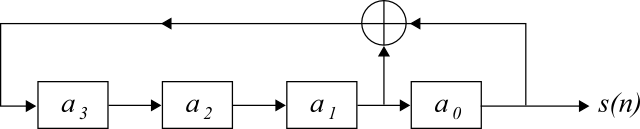
\includegraphics[width=10cm]{images/Directivity_MLS.png}
    \caption{A block diagram of a fourth order MLS, with $a_i$ the coefficients of a fourth order primitive polynomial. The addition is modulo 2 (equivalent to the exclusive-or operation).}
    \label{fig:register}
\end{figure}

This method has a good S/N ratio, which makes it suited for measurements in noisy environments. For deconvolution the fast Hadamard transform can be used, to minimize the number of computations to approximately $P\cdot\log_2(P)$ additions (where $P$ is the number of entries in the ML sequence), as described by Hee \cite{hee2003}.

There's also a variation on the MLS known as inverse repeated signal (IRS) \cite{Stan2002249}. An IRS sequence ($i[n]$) with a period of $2L$ is defined from the corresponding MLS sequence ($m[n]$) with period $L$ by the following relationship:
\[
i[n]=\left\{
\begin{array}{ll}
m[n]&\text{ if }n\text{ is even, for }0\leq n \leq 2L\\
-m[n]&\text{ if }n\text{ is odd, for }0< n < 2L\\
\end{array}
\right.
\]
The deconvolution of this signal is the same as for the ML sequence. In comparison to the MLS, the IRS signal suppresses all even harmonics, so it suffers less from distortion at those harmonics \cite{Barker1999717}.

\subsubsection{Time-stretched pulse (TSP)}
The time-stretched pulse (TSP) technique is an impulse response measurement method which was introduced by Aoshima \cite{Aoshima19811484}. It is based on specifying a wideband, spectrally flat signal, then taking the inverse Fourier transform to yield a suitable time-domain signal. If the phase of the signal is taken to be zero, an impulse-like signal results which, as discussed above, is unsuitable because of its high crest factor. The time-stretched can be considered to be the output of a phase-shifting filter applied to an impulse signal, with a transfer function given in equation \ref{eq:TSPfilter}.

\begin{equation}
H(n) = \exp[j(12n^{2}/10000)]
\label{eq:TSPfilter}
\end{equation}

This filter has a magnitude of 1, so it will conserve the wideband frequency content of the signal and only shift its phase. This added phase shift results in a stretched signal in time. The time-stretched pulse is suitable for use as a test signal because it has a better crest factor for a given energy content.

The impulse response can be recovered by using an inverse filter with transfer function (\ref{eq:TSPinversefilter}) on the Fourier transform of the received signal.

\begin{equation}
H^{-1}(n) = \exp[-j(12n^{2}/10000)]
\label{eq:TSPinversefilter}
\end{equation}

The technique of Aoshima is suitable for sound signals with small time duration. For long impulse responses, Aoshima's technique exhibits a discontinuity at frequencies over $f_{s}$/2 and below zero, which is caused by aliasing. As the transfer functions of acoustic arrangements often display long impulse responses, Suzuki et al.\ \cite{Suzuki19951119} designed the Optimized Aoshima Time Stretched Pulse technique (OATSP). They first generalized Aoshima's TSP to the function \ref{eqn:OATSPorigineel}.

\begin{equation}
\label{eqn:OATSPorigineel}
H(k)=\left\{
\begin{array}{ll}
\exp(jpk^2)& 0 \leq k < N/2\\
1&k=N/2\\
H^{*} (N-k) & N/2 < k < N
\end{array}
\right.
\end{equation}
    
Where $N=2^{i}$, with $i\in\mathbb{N}$, and the variable $p$ determines the stretch of the signal. 
The discontinuities in phase can arise because $H(N/2)$ is always set to the real value 1. To remove this discontinuity, they introduced an integer $m$ that determines the stretch of the pulse, given by equation \ref{eq:OATSPm}, which is then substituted in equation \ref{eqn:OATSPorigineel}. As can be seen from equation \ref{eq:OATSP}, this integer $m$ prevents the occurrence of $H(N/2) = 1$ and thus removes the discontinuities.

\begin{equation}
p(N/2)^{2} = m \pi
\label{eq:OATSPm}
\end{equation}

\begin{equation}
\label{eq:OATSP}
H(k)=\left\{
\begin{array}{ll}
\exp(j4m \pi k^{2}/N^{2})& 0 \leq k \leq N/2\\
H^{*} (N-k) & N/2 < k < N
\end{array}
\right.
\end{equation}
The OATSP gives an almost ideal characteristic to measure impulse responses shorter and even longer than its specific length N. 

\subsubsection{Sine-sweep}
The last method we researched is the sine-sweep method. This method differs from the other two because it assumes a linear, time-invariant system \cite{Stan2002249}. The sine-sweep method assumes that it is possible to simultaneously deconvolve the linear impulse response and to selectively separate each impulse response corresponding to the harmonic distortion orders considered.

It is relatively hard to separate the linear part from the non-linear part (associated with the distortions). In case of a logarithmic sine-sweep, the generated signal is in the form of:
\[
x(t)=\sin\left[\dfrac{T\omega_1}{\ln\left(\dfrac{\omega_2}{\omega_1}\right)}\left\{\exp\left[\dfrac{1}{T}\ln\left(\dfrac{\omega_2}{\omega_1}\right)-1\right]\right\}\right] \text{ with: }\begin{array}{l}
T \text{ duration of the sweep}\\
\omega_1 \text{ initial radian frequency}\\
\omega_2 \text{ final radian frequency}
\end{array}
\]

The deconvolution of the impulse response is realized by linearly convolving the output of the measured system with an inverse filter, given by \cite{Stan2002249}.

\subsubsection{Comparison}
Which of these three techniques is the best performing technique for determining the impulse response of a system? Stan et al.\ \cite{Stan2002249} conclude that the MLS technique is strongly immune to all kinds of noise and it has a relatively low optimal sound level. But its calibration to obtain optimal results is hard and the MLS technique is sensitive to distortion by non-linearities.

The TSP method on the other hand, is much less sensitive to these distortions, but needs much higher sound output levels to decrease the influence of noise. So it is less useful in noisy environments with respect to the MLS sequence.

Finally, the Sine-Sweep method is the best method for impulse response measurements in quiet rooms. It is insensitive to harmonic distortion and has an excellent signal-to-noise ratio. Its calibration is a lot less tedious to obtain good results, but is not recommended for measurements in noisy environments.

%-------------------------------------------------------------------------
\subsection{Sampling and interpolation methods on a sphere}
Sampling and interpolation methods on a sphere are rooted in nontrivial mathematics \cite{Marzo2014}. Zhang et al.\ \cite{Zhang2012575} show that there exists a minimum number of measurement points $M$ (formula \ref{eqn:minimum}) on a sphere.
\begin{equation}
\label{eqn:minimum}
M\equiv\left\lceil\left(\dfrac{e\pi sf}{c}+1\right)^2\right\rceil
\end{equation}
With $e=\exp(1)$, $s$ the radius of the sphere, $f$ the highest frequency and $c$ speed of sound.

\begin{figure}[b!]
    \centering
    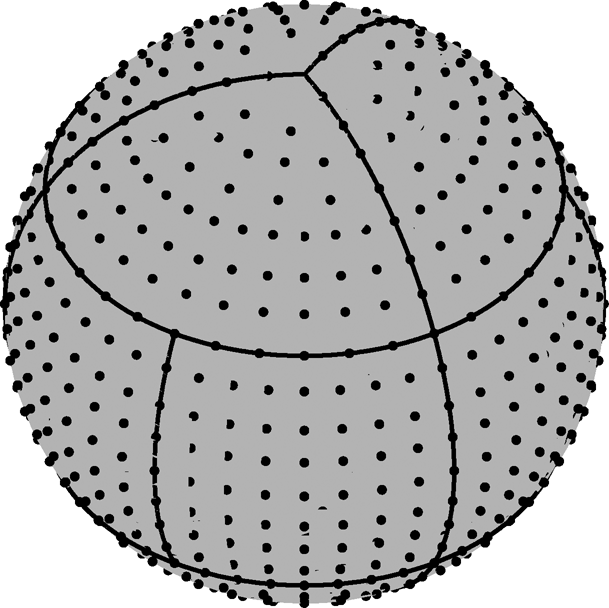
\includegraphics[width=5cm]{images/Directivity_IGLOO.png}
    \caption{An example of a IGLOO sampling scheme, Fig. 1 from \cite{Zhang2012575}. \textit{Picture of the 3:6:3 equal area division, which divides the sphere into 12 base regions, three at either cap and six $60^\circ\times60^\circ$ equatorial regions. Here, each base region is sampled with 64 points.}}
    \label{fig:IGLOO}
\end{figure}

Zhang et al.\ \cite{Zhang2012575} also describe and compare four different sampling schemes for a sphere: three existing sampling schemes and one developed by Zhang et al.\ \cite{Zhang2012575}, IGLOO, an example of the distribution of sampling points on a sphere using the IGLOO method can be found in Figure \ref{fig:IGLOO}, for which they took in consideration that it is desirable to keep the rotations to a minimum number of steps \cite{Zhang2012575}. Their results are given in Table \ref{tab:IGLOO}.

\begin{itemize}
\item[]	\textbf{Equiangular grid} is a grid equally divided in latitude and longitude. The biggest drawback is the overly densely sampled pole-region, which is reflected in the high number of samples needed compared with the ideal number.
\item[]	\textbf{Gauss-Legendre sampling} takes the points as roots of the Legendre polynomial and corresponding weights are determined by the Gauss-Legendre method. The downside of this method is that there is no regularity in the sampling region and that the sampling grids for different resolutions are completely dissimilar. As such, a lower-resolution sampling grid cannot simply be taken as a subset of a higher-resolution grid.
\item[]	\textbf{HEALPix} requires a lot of sample points with respect to the other three sampling methods and the stated minimum (equation \ref{eqn:minimum}). Also, the azimuthal positions change with the elevation.
\item[]	\textbf{IGLOO} divides the sphere into a number of base regions subject to a minimum distortion criterion. The data posseses an exact dicrete azimuthal symmetry which allows fast and precise spherical harmonic transform computation. The sample locations are more suitable for automatic measurement.
\end{itemize}

\begin{table}[t!]
\centering
\begin{tabular}{ccccc}
\hline
\hline
&Equiangular&Gauss-Legendre&HEALPix&IGLOO\\
\hline
Number of samples (for 20 kHz bandwidth)&8836&4371&12288&3072\\
Equal area division&No&No&Yes&Almost\\
Hierarchical&Yes&No&Yes&Yes\\
Iso-longitude&Yes&Yes&No&No\\
\hline
\hline
\end{tabular}
\caption{Comparison between four different methods for sampling on a sphere, Table I from \cite{Zhang2012575}. The ideal number of samples is 2209.}
\label{tab:IGLOO}
\end{table}